% !TEX encoding = UTF-8
% !TEX TS-program = pdflatex
% !TEX root = ../main.tex
% !TEX spellcheck = en-EN

%************************************************


\section{Plant Phenotyping} % parlare del plant phenotyping in generale e i suoi utilizzi in ambito pratico
Plant phenotyping, i.e. the visual analysis of the morphological and functional characteristics of a plant, is a fundamental part of the improvement process
quantitative and qualitative of plants of agricultural interest. It is connected to genomics with the analysis of the phenotype or with the performance of plants during
interaction with environmental stimuli. From the analysis of the phenotype derives a better understanding of the plant-environment system, with the possibility of setting
innovative breeding programs for new varieties. The new generation DNA sequencing techniques have revolutionized the methods and timing of selection in agricultural
species, facilitating the genetic investigation of the characters, the identification of allele genes responsible for phenotypic expression and the
their consequent transfer into new varieties through assisted selection with the use of molecular markers and the application of genomic selection.

Phenotyping emerges as a major limiting factor in the process of understanding the genetic, physiological and biochemical basis of agronomic traits, not only because of
the high cost involved and the large margin of error, but also because of the large amount of time required to collect all the necessary data. This is the reason why
in recent years there has been a growing interest in the technical and scientific world in the development of high-throughput phenotyping platforms, i.e. fully
automated plants in greenhouses or growth chambers, equipped with precise environmental control and remote sensing techniques to assess plant growth and performance.
This has been made possible by advances in engineering and computing, and the increased availability of hardware to store data at relatively low cost
In particular, the availability of new sensors based on different image acquisition systems (visible, thermal and spectral at different wavelengths, distance),
as well as the development of robotics and unmanned aerial vehicles or drones, together with the development of dedicated development of dedicated processing software,
facilitates the acquisition of data for features of interest on a large scale, in a precise, accurate, rapid and low-cost manner. Generally, these robotic and computerized
platforms acquire and analyse images in the visible light (RGB, RGBD) to perform analyses on morphology, architecture, colour, health and phenological stage of the crop.


\section{Instance segmentation}% parlare della instance segmentation e dei suoi utilizzi
Computer vision problems include: image classification, object detection and object segmentation. In order to solve these problems, deep machine learning deep machine
learning techniques are used to solve these problems. If in image classification, the classes to which the objects in an image belong are indicated, in object detection
in an image, object detection identifies the object and indicates its position.

\begin{figure}[h]
    \centering
    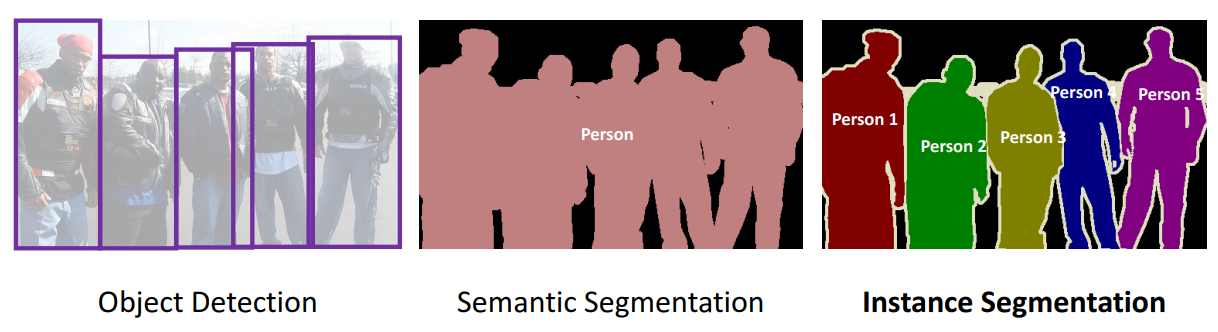
\includegraphics[width=1\textwidth]{yolact}
    \caption{Difference between object detection, semantic segmentation and instance segmentation}
\end{figure}

On the other hand, image segmentation is the technique which, during the processing and
analysis of digital images, makes it possible to divide an image into parts or regions, often on the basis of pixel characteristics. This technique was mainly developed
to effectively solve problems and critical issues that require detailed information about the objects in an image. Details that cannot be provided at all by classifying
the entire image or parts of it corresponding to a simple box. An important process This important process only ends when the objects, or rather the regions of interest,
have been identified and we move on to the extraction and analysis of the information obtained.
There are two different types of segmentation, the semantic segmentation based on the type of object present, in which all pixels belonging to a type of object are
classified in the same way and marked with a single pixel colour. In contrast, instance-based segmentation derives from the first but differs in that object detection
is also applied to the elements present in the image and each object is classified and instantiated in its own class with a different label.


\section{Thesis goal}
The aim of this thesis is to apply new methods in the field of deep learning to plant phenotyping and to demonstrate how machine learning can accurately identify plant
phenotypic traits and extrapolate their characteristics in order to quickly and accurately help plant breeders to identify plant phenotypes. identify precisely the
phenotypic traits of plants and extrapolate their characteristics in such a way as to help the farmer, the agronomist or the technician in charge of the plant phenotyping
in a fast and precise way. the farmer, agronomist or technician who will manage the plantation. The state of the art will be analysed and it will be illustrated how the
data collection and comparison of the data was carried out. The state of the art will be analysed and it will be explained how to collect data and compare results:
\begin{itemize}
    \item Analysing the state of the art and performance of neural networks with regard to plant phenotyping;
    \item Choosing which networks perform best, implementing them and training them on existing datasets; 
    \item Recreating a controlled environment where measurements can be tested and extrapolated for verification;
\end{itemize}


\section{Thesis structure}
This thesis is structured in five chapters.

The first, as we have just seen, is an introduction to the problem and the techniques that will be used.

The second chapter describes the main articles related to the problem, their approach with different resolutions and their results.

In the third chapter, we present our solution to the problem, how it should be approached, what are the best neural networks that fit the problem and metrics used
for comparisons. the problem and the metrics used for comparisons.

In the fourth chapter, the datasets are presented. In particular, the datasets used for training the networks are shown, followed by the calculation of the metrics
and the comparison with other state-of-the-art methods. the calculation of the metrics and then the comparison with the other methods seen in the state of the art.
Finally, we show our dataset, how it was acquired and its main characteristics, as well as the experimental results collected both by direct measurement and by the
proposed solution. Finally, the metrics related to our dataset are shown.

In the fifth and final chapter, conclusions and possible future developments are discussed.





